\subsection{Hadoop Filesystem}

Hadoop filesystem (HDFS) is a distributed filesystem that seeks to increase fault tolerance on very large datasystems. The filesystem is designed to be distributed across inexpensive commodity hardware, where recovery is done quickly and automatically. HDFS is run on a cluster, where one machine exist as a name node, which is a central node that manages the location of file blocks. Blocks are used as a means to split large files, replicate and distribute them across the cluster’s data nodes. Naturally, ensuring file coherency could become very complicated in such a system, which is why Hadoop implements a simple “write once read many” model. Commonly the file sizes used with Hadoop is in the Gigabyte-Terabyte range.
Looking at \cref{hadoop}, the name node can be seen as the root of a HDFS cluster. An application access data by first requesting the locations of a file’s blocks from the name node and then use those locations to read directly from data nodes. As described earlier the cluster used for for the work in this article, consists of the centreal name node and three data nodes.~\cite{hadoopIntro} 

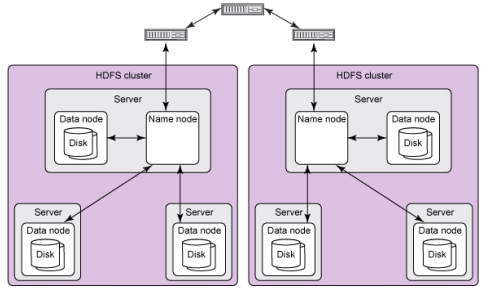
\includegraphics[scale=1]{images/hadoopoverview.png} \label{hadoop} 